\documentclass{beamer}
\usepackage[utf8]{inputenc}
\usetheme{Madrid}
\usecolortheme{default}
\usepackage{amsmath,amssymb,amsfonts,amsthm}
\usepackage{txfonts}
\usepackage{tkz-euclide}
\usepackage{listings}
\usepackage{adjustbox}
\usepackage{array}
\usepackage{tabularx}
\usepackage{gvv}
\usepackage{lmodern}
\usepackage{circuitikz}
\usepackage{tikz}
\usepackage{graphicx}

\setbeamertemplate{page number in head/foot}[totalframenumber]

\usepackage{tcolorbox}
\tcbuselibrary{minted,breakable,xparse,skins}



\definecolor{bg}{gray}{0.95}
\DeclareTCBListing{mintedbox}{O{}m!O{}}{%
  breakable=true,
  listing engine=minted,
  listing only,
  minted language=#2,
  minted style=default,
  minted options={%
    linenos,
    gobble=0,
    breaklines=true,
    breakafter=,,
    fontsize=\small,
    numbersep=8pt,
    #1},
  boxsep=0pt,
  left skip=0pt,
  right skip=0pt,
  left=25pt,
  right=0pt,
  top=3pt,
  bottom=3pt,
  arc=5pt,
  leftrule=0pt,
  rightrule=0pt,
  bottomrule=2pt,
  toprule=2pt,
  colback=bg,
  colframe=orange!70,
  enhanced,
  overlay={%
    \begin{tcbclipinterior}
    \fill[orange!20!white] (frame.south west) rectangle ([xshift=20pt]frame.north west);
    \end{tcbclipinterior}},
  #3,
}
\lstset{
    language=C,
    basicstyle=\ttfamily\small,
    keywordstyle=\color{blue},
    stringstyle=\color{orange},
    commentstyle=\color{green!60!black},
    numbers=left,
    numberstyle=\tiny\color{gray},
    breaklines=true,
    showstringspaces=false,
}
%------------------------------------------------------------
%This block of code defines the information to appear in the
%Title page
\title %optional
{4.4.33}

%\subtitle{A short story}

\author % (optional)
{stalin-ai25btech11037}



\begin{document}


\frame{\titlepage}
\begin{frame}{Question}
\text{Find the value of } x \text{ such that the four points with position vectors } $\vec{A}(3\hat{i} + 2\hat{j} + \hat{k}), \vec{B}(4\hat{i} + x\hat{j} + 5\hat{k}), \vec{C}(4\hat{i} + 2\hat{j} - 2\hat{k}), \text{ and } \vec{D}(6\hat{i} + 5\hat{j} - \hat{k})$ \text{ are coplanar.} \quad (12, 2018)\\ 
\end{frame}



\begin{frame}{Theoretical Solution}
Let us solve the given equation theoretically and then verify the solution computationally \\
According to the question, \\
Given four position vectors\\
\begin{align}
    \vec{A}=\begin{myvec}{3\\2\\1}\end{myvec}\
    \vec{B}=\begin{myvec}{4\\x\\5}\end{myvec}\
    \vec{C}=\begin{myvec}{4\\2\\-2}\end{myvec}\
    \vec{D}=\begin{myvec}{6\\5\\-1}\end{myvec}\
\end{align}
\begin{align}
    \vec{A}^T\vec{n}=1
\end{align}
\begin{align}
    \vec{B}^T\vec{n}=1
\end{align}
\begin{align}
    \vec{C}^T\vec{n}=1
\end{align}


\end{frame}

\begin{frame}{Theoretical Solution}
\begin{align}
    \vec{D}^T\vec{n}=1
\end{align}
\begin{align}
    \begin{myvec}{A&&B&&C&&D}^T\end{myvec}\vec{n}=\begin{myvec}{1\\1\\1\\1}\end{myvec}
\end{align}
Let 
\begin{align}
    \vec{i}=\myvec{1\\1\\1\\1}\
    \vec{z}=\begin{myvec}{A&&B&&C&&D}^T\end{myvec}
\end{align}
condition is Rank of $\begin{myvec}{A&&B&&C&&D}^T\end{myvec}$=3
and $\begin{myvec}{z&&i}\end{myvec}$=3\\
From solving we get x=5.
\end{frame}



\begin{frame}[fragile]
    \frametitle{C Code }

    \begin{lstlisting}
#include <stdio.h>

// Function to calculate the scalar triple product condition for coplanarity
double scalar_triple_product_condition(double x) {
    // Components of vectors AB, AC, AD based on x
    // A = (3, 2, 1)
    // B = (4, x, 5)
    // C = (4, 2, -2)
    // D = (6, 5, -1)

    // AB = B - A = (1, x-2, 4)
    double AB_x = 1;
    double AB_y = x - 2;
    double AB_z = 4;

    // AC = C - A = (1, 0, -3)
    double AC_x = 1;
    double AC_y = 0;
    

     \end{lstlisting}
\end{frame}
\begin{frame}[fragile]
    \frametitle{C Code }

    \begin{lstlisting}
   double AC_z = -3;

    // AD = D - A = (3, 3, -2)
    double AD_x = 3;
    double AD_y = 3;
    double AD_z = -2;

    // Cross product AC x AD
    double cross_x = AC_y * AD_z - AC_z * AD_y; // 0*(-2) - (-3)*3 = 9
    double cross_y = AC_z * AD_x - AC_x * AD_z; // (-3)*3 - 1*(-2) = -7
    double cross_z = AC_x * AD_y - AC_y * AD_x; // 1*3 - 0*3 = 3

    // Dot product AB . (AC x AD)
    double scalar_triple = AB_x * cross_x + AB_y * cross_y + AB_z * cross_z;

    \end{lstlisting}
\end{frame}
\begin{frame}[fragile]
    \frametitle{C Code }

    \begin{lstlisting}
    
    return scalar_triple;
}

int main() {
    // From the math, we have linear equation 35 - 7x = 0 => x = 5
    // But let's also verify numerically:

    double x = 5.0;
    double result = scalar_triple_product_condition(x);

    printf("Value of x for coplanarity: %.2f\n", x);
    printf("Scalar triple product at x=%.2f: %.2f (should be close to 0)\n", x, result);

    return 0;
}

    \end{lstlisting}
\end{frame}
\begin{frame}[fragile]
    \frametitle{Python Code}
    \begin{lstlisting}
import numpy as np
import matplotlib.pyplot as plt
from mpl_toolkits.mplot3d import Axes3D

# Given vectors (with x unknown)
# A = 3i + 2j + k
A = np.array([3, 2, 1])

# Solve for x such that points are coplanar

# Let x be the unknown coordinate in B's j component and k component
# B = 4i + xj + 5k
# C = 4i + 2j - 2k
# D = 6i + 5j - k

# Set up vectors AB, AC, AD
def scalar_triple_product(x):
    B = np.array([4, x, 5])
   

  





    \end{lstlisting}
\end{frame}

\begin{frame}[fragile]
    \frametitle{Python Code}
    \begin{lstlisting}
     C = np.array([4, 2, -2])
    D = np.array([6, 5, -1])
  AB = B - A
    AC = C - A
    AD = D - A

    return np.dot(AB, np.cross(AC, AD))

# Solve for x using the derived formula or by root finding
from scipy.optimize import fsolve

x_solution = fsolve(scalar_triple_product, 0)[0]

# Recalculate B with the found x
B = np.array([4, x_solution, 5])
C = np.array([4, 2, -2])
D = np.array([6, 5, -1])

# 3D plot


    \end{lstlisting}
\end{frame}

\begin{frame}[fragile]
    \frametitle{Python Code}
    \begin{lstlisting}
fig = plt.figure(figsize=(8,6))
ax = fig.add_subplot(111, projection='3d')
# Plot points
ax.scatter(*A, color='r', label='A')
ax.scatter(*B, color='g', label=f'B (x={x_solution:.2f})')
ax.scatter(*C, color='b', label='C')
ax.scatter(*D, color='purple', label='D')

# Draw vectors from origin for clarity
for vec, name, color in zip([A, B, C, D], ['A', 'B', 'C', 'D'], ['r', 'g', 'b', 'purple']):
    ax.text(vec[0], vec[1], vec[2], f'{name}', size=12, color=color)

# Plot the plane defined by A, C, D (since points are coplanar)
# Plane normal vector
normal = np.cross(C - A, D - A)
    \end{lstlisting}
\end{frame}
\begin{frame}[fragile]
    \frametitle{Python Code}
    \begin{lstlisting}
   # Create a grid of points on the plane
d = -np.dot(normal, A)
xx, yy = np.meshgrid(np.linspace(2, 7, 10), np.linspace(0, 6, 10))
zz = (-normal[0] * xx - normal[1] * yy - d) / normal[2]

ax.plot_surface(xx, yy, zz, alpha=0.3, color='cyan')

ax.set_xlabel('X')
ax.set_ylabel('Y')
ax.set_zlabel('Z')
ax.set_title('Coplanar Points A, B, C, D')

ax.legend()
plt.savefig('coplanar_points.png')
plt.show()
 \end{lstlisting}
\end{frame}
\begin{frame}{Plot}
    \centering
    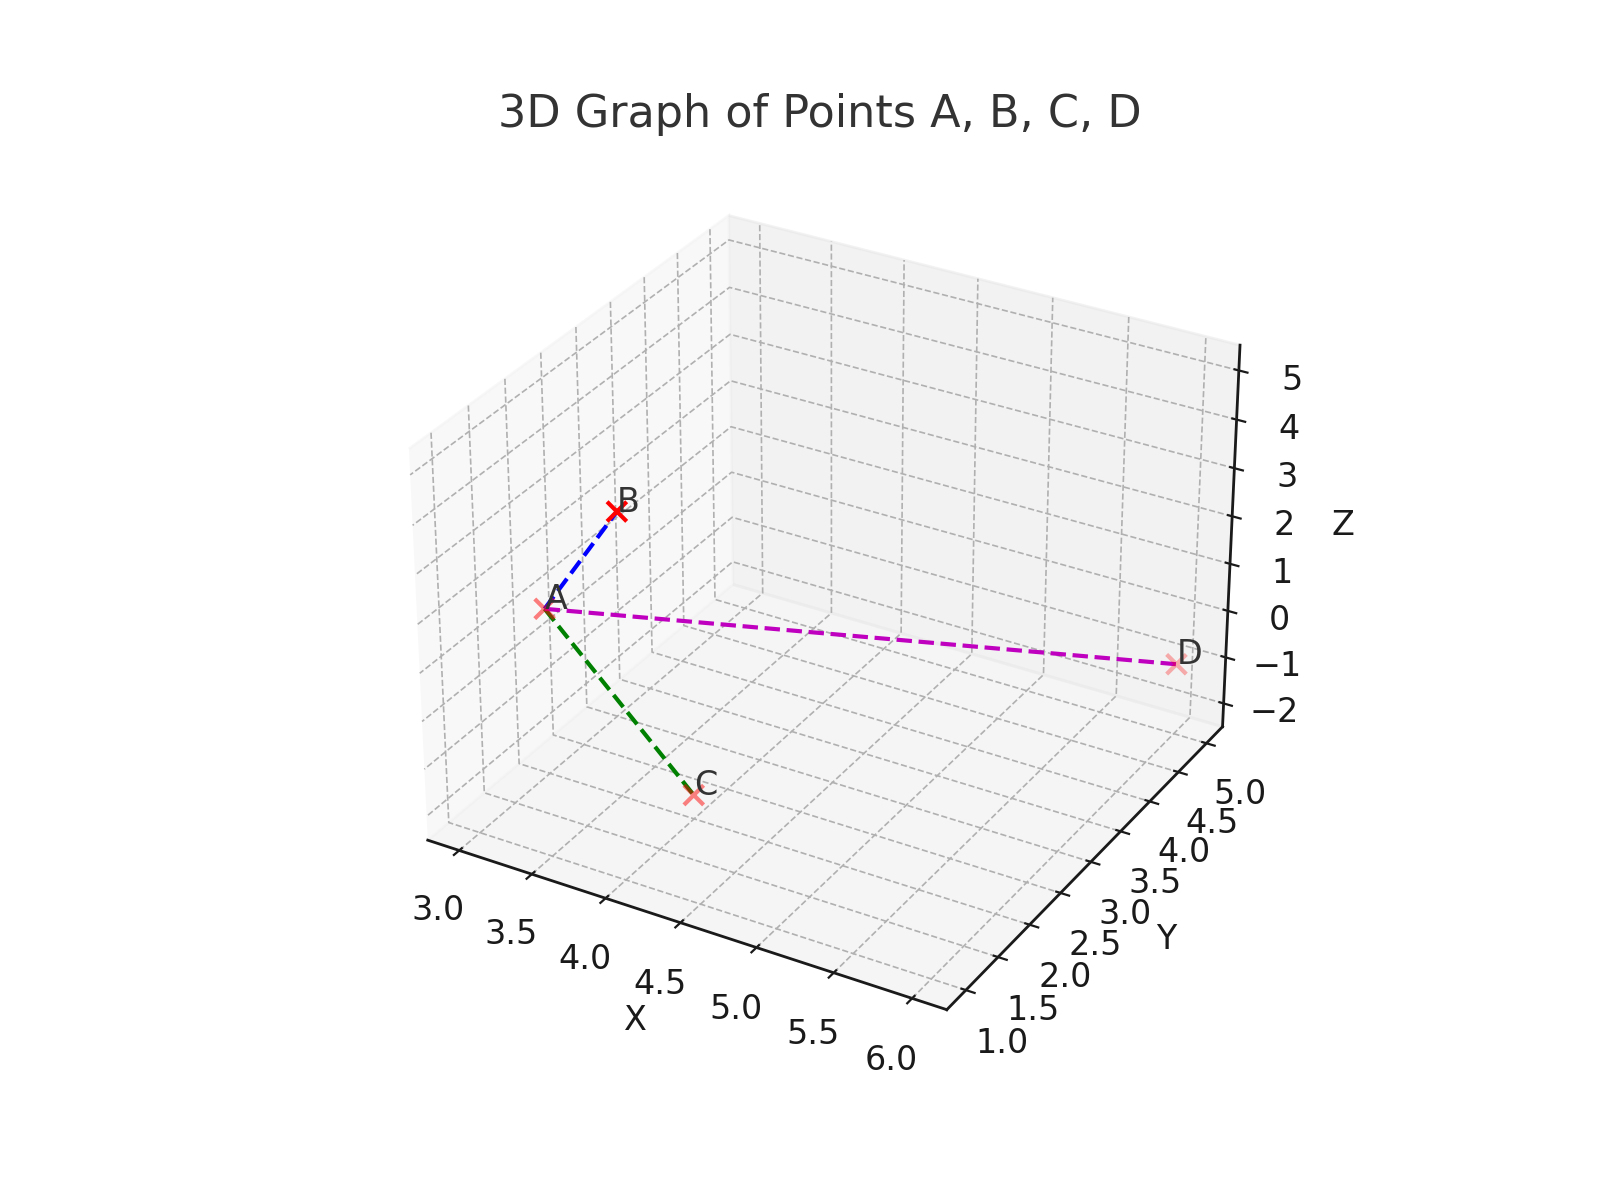
\includegraphics[width=\columnwidth, height=0.8\textheight, keepaspectratio]{figs/3D_points_plot.png}     
\end{frame}




\end{document}